\chapter{Strumenti di Sincronizzazione}
Nei capitoli precedenti abbiamo visto che più processi possono eseguire parallelamente, crando però diversi problemi, come la \textbf{race condition}.
Per evitare situazioni come questa, è necessario usare metodi di sincronizzazione o di coordinazione.

\section{Problema della Sezione Critica}
Ipotizziamo di avere $n$ processi $[P_1, P_2, \dots, P_n]$, in cui ognuno di questi abbia una parte critica,
ovvero una parte in cui deve usare dei dati condivisi con altri processi senza che nessuno li modifichi. \\ 
Generalmente, è necessario un metodo per sincronizzare i processi, magari mettendo in evidenza l'inzio e la fine di un sezione di codice critica, dividendola così dal codice restante.

\begin{figure}[!htb]
    \centering
    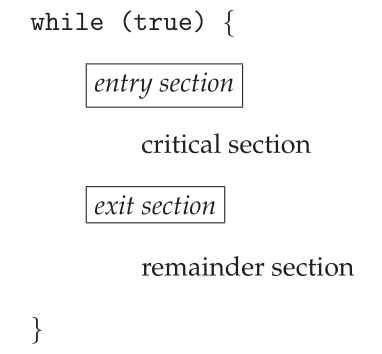
\includegraphics[width=0.3\linewidth]{Images/syncro/critical.png}
  \caption{Sezione Critica.}
\end{figure}

Le soluzioni a questo problema devono rispettare queste tre caratteristiche:
\begin{enumerate}
  \item \textbf{Mutual Exclusion:} se il processo $P_i$ sta eseguendo la sua sezione critica, allora nessun altro processo può eseguire la propria zona critica.
  \item \textbf{Progresso:} se nessun processo sta eseguendo la sua zona critica, ma alcuni vorrebbero, allora la selezione di questo processo non può essere spostata all'infinito.
  \item \textbf{Bounded Waiting:} deve esistere un limite al numero di volte in cui ad altri processi è consentito entrare nelle proprie sezioni critiche dopo che un processo ha inoltrato una richiesta di accesso alla propria sezione critica.
\end{enumerate}

\subsection{Prime Soluzioni Software}
Nel caso di un sistema singlecore, il problema della sezione critica si può evitare disabilitando l'arrivo delle interrupts, potendo così eseguire il codice in tranquillitaà. 
Ovviamente, questa soluzione ha diversi limiti, sopratutto il fatto che i computer moderni sono quasi tutti multicore, dove disabilitare le interrupt protrebbe rallentare il sistema.
Generalmente, esistono due altri approcci possibili:
\begin{enumerate}
  \item \textbf{Non-Preemtive Kernels:} non permette ai processi che eseguo in kernel mode di essere cambiati con un altro. Questo evita del tutto le race condition.
  \item \textbf{Preemtive Kernels:} i processi che eseguo in kernel mode possono essere cambiati, creando possibili race condition. I sistemi, però, sono più fluidi e responsivi.
\end{enumerate}

\subsection{Soluzione di Peternson}
Soluzione software classica per risolvere il problema della sezione critica, in particolare questa soluzione risolve il problema di due processi che si alternano nell'esecuzione.
Ipotizziamo di avere due processi $P_0$ e $P_1$, due varibili condivise \texttt{int turn} che indica di chi è il turno e \texttt{boolean flag[2]} che indica se il processo è pronto per entrare nella sezione critica. 
Inoltre, si ipotizza che le istruzioni di load e di store siano atomiche:

\begin{clang}[Esempio per $P_i$ ($P_0$)]
while (true){
  flag[i] = true;
  turn = j;
  
  while (flag[j] && turn == j){}; // wait for turn i
    /* here is the critical section */
  
  flag[i] = false;
  /* here is the remainder section */
}
\end{clang}

\subsubsection{Correttezza della soluzione}
Per verificare che la soluzione si corretta:
\begin{enumerate}
  \item \textbf{Mutual Exclusion:} $P_i$ può entrare solo se è il suo turno o se $P_j$ non è pronto per entrare. \textcolor{blue}{\textbf{OK}}.
  \item \textbf{Prograss:} $P_i$ può essere bloccata in loop dall'entrare solo se $P_j$ è pronto ed è il suo turno, altrimenti, senza una di queste due condizioni può entrare. \textcolor{blue}{\textbf{OK}}.
  \item \textbf{Bounded Waiting:} stesso motivo di prima. \textcolor{blue}{\textbf{OK}}.
\end{enumerate}

In archietture moderne, dove le istruzioni senza dipendenze vengono riordinate, si potrebbero creare diversi problemi, come la situazione in cui due processi entrino entrambi nella loro sezione critica.

\begin{figure}[!htb]
    \centering
    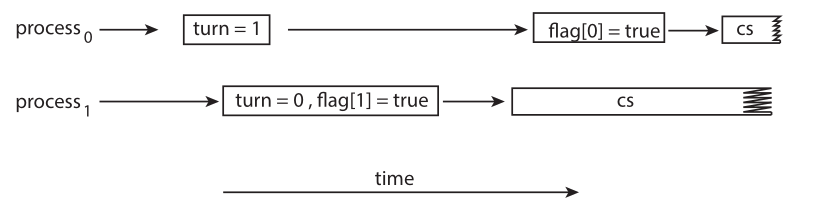
\includegraphics[width=0.5\linewidth]{Images/syncro/peterson.png}
  \caption{Sezione Critica Simultanea.}
\end{figure}

Questo problema si può risolvere con soluzione hardware, come la \textbf{memory barrier}.

\subsection{Memory Barrier}
Di solito quello che garantisce cosa la memoria provvederà a una applicazione è chiamato \textbf{modello della memoria}, ne esitono di due tipi:
\begin{enumerate}
  \item \textbf{Strongly Ordered:} quando la modifica della memoria da parte di un processo è immediatamente visibile agli altri processi.
  \item \textbf{Weakly Oredered:} quando la modifica della memoria da parte di un processo può non essere immediatamente visibile agli altri processi.
\end{enumerate}

Varia a seconda del tipo di processore, quindi non possono essere fatte assunzioni a livello kernel. \\ 
Per questo, per evitare problemi, vengono create delle istruzioni che forzano che un cambiamento della memoria si propaghi su tutti i processi.

\begin{defn}[Memory Barrier]
Conosciuta anche come \textbf{memory fence}, è un'istruzione che impone che qualsiasi modifica in memoria venga propagata a tutti gli altri processori.
In caso di riordinamento delle istruzioni, questa tecnica permette di di assicurare che le azioni vengano mostrate a tutti i processi.
\end{defn}

Questo permette a tutte le istruzioni di load e store di essere completate e visibili.

\begin{clang}[Esempi con Thread 1 e 2]
# Thread 1
while (!flag)
  memory barrier();
print x;

# Thread 2
x = 100;
memory_barrier();
flag = true;
\end{clang}

\subsection{Istruzioni Hardware}
Molti sistemi moderni mettono a disposizione delle istruzioni a livello hardware che permetto di modificare o sostituire il contenuto di una variabile atomicamente,
ossia senza che possa essere fermata per nessun motivo. \\
\vspace*{0.01\textheight}
Esistono due istruzioni principali:
\begin{enumerate}
  \item \texttt{test\_and\_set()}.
  \item \texttt{compare\_and\_swap()}.
\end{enumerate}
\begin{clang}[test\_and\_set()]
boolean test_and_set(boolean *target) {
  boolean rv = *target;
  *target = true;
  
  return rv;
}
\end{clang}
\begin{clang}[compare\_and\_swap()]
do {
  while (test_and_set(&lock))
    ; /* do nothing */
  /* critical section */
  lock = false;
  /* remainder section */
} while (true);
\end{clang}

Questo esempio assicura sicuramente l'esclusione mutua, ma è possibile pure garantire il progresso e il bounded waiting.

\begin{clang}[Esempio per Bounded Waiting]
while (true) {
  waiting[i] = true;
  key = 1;
  while (waiting[i] && key == 1){
    key = compare_and_swap(&lock,0,1)
  }

  waiting[i] = false;
  /* here is the critical section */
  j = (i + 1) % n;
  
  while ((j != i) && !waiting[j]){
    j = (j + 1) % n;
  }

  if (j == i)
    lock = 0;
  else
    waiting[j] = false;

  /* here is the remainder section */
}
\end{clang}

All'interno dell'ISA x86 esiste lo statement \texttt{cmpxchg} con il prefisso \texttt{lock}, per implementare l'istruzione \texttt{compare\_and\_swap()} in modo atomico.
La forma generale risulta del tipo:
\[
  \text{\texttt{lock cmpxchg <destination operand>, <source operand>}}
\]
\begin{defn}[Variabili Atomiche]
Le variabili atomiche consentono aggiornamenti atomici, quindi non interrompibili, su tipi di dati di base, come interi e booleani.
\end{defn}
Solitamente, istruzioni come \texttt{compare\_and\_swap()}, non vengono usate direttamente, ma piuttosto servono a creare costrutti utili a risolvere il probelma delle sezioni critiche. \\
Immaginiamo di avere una variabile atomica \texttt{sequence} e una funziona che che opera su varibaili atomiche \texttt{increment()}:
\begin{clang}[Esempio di uso di Varibaili Atomiche]
void increment(atomic_int *v){
  int temp;
  do {
    temp = *v;
  } while (temp != (compare_and_swap(v,temp,temp+1)));
}
\end{clang}
